\documentclass[a3paper,12pt]{extarticle} % Use extarticle for A3 paper size
\usepackage{graphicx} % Include this package for \includegraphics
\usepackage{amsmath}
\usepackage{amssymb} % Include this package for \mathbb
\usepackage[margin=1in]{geometry} % Adjust the margin as needed
\usepackage{float}


\begin{document}

\author{kipngeno koech - bkoech}
\title{Homework 4 - Introduction to Probabilistic Graphical Models}   
\maketitle

\medskip

\maketitle

\section{Structure Learning}
\subsection{Tree-Selection and the Chow-Liu Algorithm}
Use the Chow-Liu Algorithm to learn the model (tree and parameters) that generated the following data.

\begin{figure}[H]
\centering
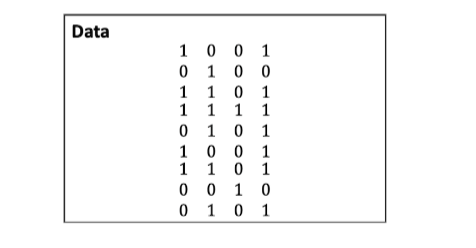
\includegraphics[width=0.8\textwidth]{q1.png}
\caption{The tree structure of the data.}
\label{fig:tree}
\end{figure}

\subsection{Scoring Function}
Using the BIC scoring metrics below, compute the model (graph and potentials) that generated the data below. 

\textbf{BIC:}
\[
S(G, \theta; D) = LL(\theta; D) - \phi(|D|)\|G\| \quad \text{where} \quad \phi(t) = \frac{\log(t)}{2}
\]

\textbf{Maximizing the score:}
\[
S_{\text{max}}(G, D) = \max_{\theta} \big(S(G, \theta; D)\big)
\]

\begin{figure}[H]
\centering
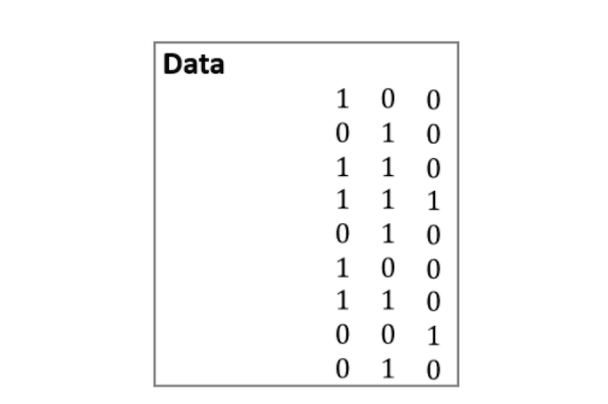
\includegraphics[width=0.8\textwidth]{q2.png}
\caption{The data used to compute the BIC score.}
\label{fig:data}
\end{figure}

\newpage
\section{Variational Inference}
\subsection{Mean-Field Approximation for Multivariate Gaussians}
In this question, we’ll explore how accurate a Mean-Field approximation can be for an underlying multivariate Gaussian distribution. Assume we have observed data \( X \in \mathbb{R}^{2 \times n} \) where each column \( X_{\cdot,i} \triangleq x^{(i)} \in \mathbb{R}^2 \) is a sample that was drawn from a 2-dimensional Gaussian distribution \( x^{(i)} \sim p(\cdot; \mu, \Lambda^{-1}) \).

\[
p(x; \mu, \Lambda) = \mathcal{N} \left( 
\begin{bmatrix}
x_1 \\
x_2
\end{bmatrix}
;
\begin{bmatrix}
\mu_1 \\
\mu_2
\end{bmatrix}
,
\begin{bmatrix}
\Lambda_{11} & \Lambda_{12} \\
\Lambda_{21} & \Lambda_{22}
\end{bmatrix}^{-1}
\right)
\tag{1}
\]

Note here that we’re using the precision matrix \( \Lambda = \Sigma^{-1} \). An additional property of the precision matrix is that it is symmetric, so \( \Lambda_{12} = \Lambda_{21} \). (This is a convenient simplifying assumption.) We will approximate this 2-dimensional Gaussian with a mean field approximation, \( q(x) = q(x_1)q(x_2) \), the product of two 1-dimensional distributions \( q(x_1) \) and \( q(x_2) \). For now, we won’t assume any form for these distributions.

\begin{enumerate}
    \item \textbf{Short Answer:} Write down the equation for \( \log p(X) \). (For this question, you can leave all of the parameters in terms of vectors and matrices, not their subcomponents.)
    \item \textbf{Short Answer:} Group together everything that involves \( X_1 \) and remove anything involving \( X_2 \). We claim that there exists some distribution \( q^*(X) = q^*(X_1)q^*(X_2) \) that minimizes the KL divergence \( q^* = \arg\min_q \text{KL}(q \| p) \). Furthermore, said distribution will have a component \( q^*(X_1) \) that will be proportional to the quantity you find below. Write that term that is proportional to \( q^*(X_1) \).
    \\\\ It can be shown that this implies that \( q(X_1) \) (and therefore \( q(X_2) \)) is a Gaussian distribution:
    \[
    q(x_1) = \mathcal{N} \left( x_1; m_1, \Lambda_{11}^{-1} \right)
    \]
    where 
    \[
    m_1 = \mu_1 - \Lambda_{11}^{-1} \Lambda_{12} \big(E[x_2] - \mu_2\big)
    \]
    Using these facts, we’d like to explore how well our approximation can model the underlying distribution.
    \item Suppose the parameters of the true distribution are 
    \[
    \mu = 
    \begin{bmatrix}
    0 \\
    0
    \end{bmatrix}
    \quad \text{and} \quad
    \Lambda = 
    \begin{bmatrix}
    1 & 0 \\
    0 & \frac{1}{4}
    \end{bmatrix}.
    \]
    
        \begin{enumerate}
            \item[(a)] \textbf{Numerical Answer:} What is the value of the mean of the Gaussian for \( q^*(X_1) \)?
            \item[(b)] (2 points) \textbf{Numerical Answer:} What is the value of the variance of the Gaussian for \( q^*(X_1) \)?
            \item[(c)] (2 points) \textbf{Numerical Answer:} What is the value of the mean of the Gaussian for \( q^*(X_2) \)?
            \item[(d)] (2 points) \textbf{Numerical Answer:} What is the value of the variance of the Gaussian for \( q^*(X_2) \)?
            \item[(e)] (5 points) \textbf{Plot:} Provide a computer-generated contour plot to show the result of our approximation \( q^*(X) \) and the true underlying Gaussian \( p(X; \mu, \Lambda) \) for the parameters given above.
        \end{enumerate}
\end{enumerate}

\end{document}